%==========================================================
% PART 5: from rain maps to flood risk (Phase 5).
%==========================================================
\par
% generated by scripts/phase5/export_explainer_phase5.py
\newcommand{\PfiveAlgAlarmHa}{5}%
\newcommand{\PfiveAlgBasinArea}{9.1}%
\newcommand{\PfiveAlgBasinRef}{10.2}%
\newcommand{\PfiveAlgBudgetErr}{2\times10^{-5}}%
\newcommand{\PfiveAlgBuilt}{56\%}%
\newcommand{\PfiveAlgCN}{85}%
\newcommand{\PfiveAlgCellX}{25}%
\newcommand{\PfiveAlgCellY}{31}%
\newcommand{\PfiveAlgCells}{0.77}%
\newcommand{\PfiveAlgCommuneAHa}{68}%
\newcommand{\PfiveAlgCommuneA}{El Harrach}%
\newcommand{\PfiveAlgCommuneBHa}{26}%
\newcommand{\PfiveAlgCommuneB}{Bachdjarah}%
\newcommand{\PfiveAlgCommuneCHa}{24}%
\newcommand{\PfiveAlgCommuneC}{Kouba}%
\newcommand{\PfiveAlgDurA}{1}%
\newcommand{\PfiveAlgDurB}{3}%
\newcommand{\PfiveAlgDurC}{6}%
\newcommand{\PfiveAlgDurD}{12}%
\newcommand{\PfiveAlgDurE}{24}%
\newcommand{\PfiveAlgFactor}{3.64}%
\newcommand{\PfiveAlgGAIAlarm}{9 Nov 22:05}%
\newcommand{\PfiveAlgGAICSI}{0.81}%
\newcommand{\PfiveAlgGAIFlood}{9 Nov 22:01}%
\newcommand{\PfiveAlgGAILead}{36\,min late}%
\newcommand{\PfiveAlgGAIModelLead}{37\,min late}%
\newcommand{\PfiveAlgGAIPeakErr}{-49\%}%
\newcommand{\PfiveAlgGAIPeakTime}{10 Nov 03:32}%
\newcommand{\PfiveAlgGAIPeak}{32}%
\newcommand{\PfiveAlgGAIQR}{0.99}%
\newcommand{\PfiveAlgGAISig}{171}%
\newcommand{\PfiveAlgGAISpear}{0.92}%
\newcommand{\PfiveAlgGAITop}{4}%
\newcommand{\PfiveAlgGAIVolErr}{-45\%}%
\newcommand{\PfiveAlgGAIVol}{1.01}%
\newcommand{\PfiveAlgGAIWet}{1{,}067}%
\newcommand{\PfiveAlgGClAlarm}{9 Nov 20:05}%
\newcommand{\PfiveAlgGClCSI}{0.86}%
\newcommand{\PfiveAlgGClFlood}{9 Nov 21:08}%
\newcommand{\PfiveAlgGClLead}{1\,h\,24 early}%
\newcommand{\PfiveAlgGClModelLead}{16\,min early}%
\newcommand{\PfiveAlgGClPeakErr}{-29\%}%
\newcommand{\PfiveAlgGClPeakTime}{10 Nov 03:26}%
\newcommand{\PfiveAlgGClPeak}{44}%
\newcommand{\PfiveAlgGClQR}{1.00}%
\newcommand{\PfiveAlgGClSig}{207}%
\newcommand{\PfiveAlgGClSpear}{0.95}%
\newcommand{\PfiveAlgGClTop}{4}%
\newcommand{\PfiveAlgGClVolErr}{-18\%}%
\newcommand{\PfiveAlgGClVol}{1.50}%
\newcommand{\PfiveAlgGClWet}{1{,}192}%
\newcommand{\PfiveAlgGSatAlarm}{10 Nov 01:00}%
\newcommand{\PfiveAlgGSatCSI}{0.84}%
\newcommand{\PfiveAlgGSatFlood}{9 Nov 21:04}%
\newcommand{\PfiveAlgGSatLead}{3\,h\,31 late}%
\newcommand{\PfiveAlgGSatModelLead}{3\,h\,35 late}%
\newcommand{\PfiveAlgGSatPeakErr}{-24\%}%
\newcommand{\PfiveAlgGSatPeakTime}{10 Nov 09:05}%
\newcommand{\PfiveAlgGSatPeak}{47}%
\newcommand{\PfiveAlgGSatQR}{0.96}%
\newcommand{\PfiveAlgGSatSig}{240}%
\newcommand{\PfiveAlgGSatSpear}{0.96}%
\newcommand{\PfiveAlgGSatTop}{4}%
\newcommand{\PfiveAlgGSatVolErr}{-15\%}%
\newcommand{\PfiveAlgGSatVol}{1.56}%
\newcommand{\PfiveAlgGSatWet}{1{,}199}%
\newcommand{\PfiveAlgGSparseAlarm}{9 Nov 20:05}%
\newcommand{\PfiveAlgGSparseCSI}{0.80}%
\newcommand{\PfiveAlgGSparseFlood}{9 Nov 21:09}%
\newcommand{\PfiveAlgGSparseLead}{1\,h\,24 early}%
\newcommand{\PfiveAlgGSparseModelLead}{15\,min early}%
\newcommand{\PfiveAlgGSparsePeakErr}{-43\%}%
\newcommand{\PfiveAlgGSparsePeakTime}{10 Nov 03:20}%
\newcommand{\PfiveAlgGSparsePeak}{36}%
\newcommand{\PfiveAlgGSparseQR}{0.96}%
\newcommand{\PfiveAlgGSparseSig}{157}%
\newcommand{\PfiveAlgGSparseSpear}{0.96}%
\newcommand{\PfiveAlgGSparseTop}{3}%
\newcommand{\PfiveAlgGSparseVolErr}{-47\%}%
\newcommand{\PfiveAlgGSparseVol}{0.97}%
\newcommand{\PfiveAlgGSparseWet}{1{,}088}%
\newcommand{\PfiveAlgGTruthAlarm}{9 Nov 21:00}%
\newcommand{\PfiveAlgGTruthFlood}{9 Nov 21:29}%
\newcommand{\PfiveAlgGTruthLead}{29\,min early}%
\newcommand{\PfiveAlgGTruthModelLead}{0\,min early}%
\newcommand{\PfiveAlgGTruthPeakTime}{10 Nov 03:19}%
\newcommand{\PfiveAlgGTruthPeak}{62}%
\newcommand{\PfiveAlgGTruthSig}{303}%
\newcommand{\PfiveAlgGTruthVol}{1.84}%
\newcommand{\PfiveAlgGTruthWet}{1{,}311}%
\newcommand{\PfiveAlgGaugeTotal}{263}%
\newcommand{\PfiveAlgGridX}{1{,}260}%
\newcommand{\PfiveAlgGridY}{612}%
\newcommand{\PfiveAlgObsHi}{140}%
\newcommand{\PfiveAlgObsLo}{90}%
\newcommand{\PfiveAlgObsModel}{89}%
\newcommand{\PfiveAlgObsPeak}{143}%
\newcommand{\PfiveAlgObsVol}{1.8}%
\newcommand{\PfiveAlgPits}{71.5}%
\newcommand{\PfiveAlgSAIAlarm}{--}%
\newcommand{\PfiveAlgSAICSI}{0.65}%
\newcommand{\PfiveAlgSAIFlood}{--}%
\newcommand{\PfiveAlgSAILead}{no alarm}%
\newcommand{\PfiveAlgSAIModelLead}{no alarm}%
\newcommand{\PfiveAlgSAIPeakErr}{-68\%}%
\newcommand{\PfiveAlgSAIPeakTime}{10 Nov 10:13}%
\newcommand{\PfiveAlgSAIPeak}{3}%
\newcommand{\PfiveAlgSAIQR}{0.98}%
\newcommand{\PfiveAlgSAISig}{30}%
\newcommand{\PfiveAlgSAISpear}{0.93}%
\newcommand{\PfiveAlgSAITop}{3}%
\newcommand{\PfiveAlgSAIVolErr}{-69\%}%
\newcommand{\PfiveAlgSAIVol}{0.08}%
\newcommand{\PfiveAlgSAIWet}{148}%
\newcommand{\PfiveAlgSClAlarm}{--}%
\newcommand{\PfiveAlgSClCSI}{0.83}%
\newcommand{\PfiveAlgSClFlood}{10 Nov 08:43}%
\newcommand{\PfiveAlgSClLead}{no alarm}%
\newcommand{\PfiveAlgSClModelLead}{2\,h\,42 late}%
\newcommand{\PfiveAlgSClPeakErr}{-27\%}%
\newcommand{\PfiveAlgSClPeakTime}{10 Nov 10:10}%
\newcommand{\PfiveAlgSClPeak}{7}%
\newcommand{\PfiveAlgSClQR}{0.98}%
\newcommand{\PfiveAlgSClSig}{33}%
\newcommand{\PfiveAlgSClSpear}{0.93}%
\newcommand{\PfiveAlgSClTop}{3}%
\newcommand{\PfiveAlgSClVolErr}{-30\%}%
\newcommand{\PfiveAlgSClVol}{0.18}%
\newcommand{\PfiveAlgSClWet}{192}%
\newcommand{\PfiveAlgSSatAlarm}{10 Nov 13:00}%
\newcommand{\PfiveAlgSSatCSI}{0.85}%
\newcommand{\PfiveAlgSSatFlood}{10 Nov 09:05}%
\newcommand{\PfiveAlgSSatLead}{6\,h\,54 late}%
\newcommand{\PfiveAlgSSatModelLead}{6\,h\,59 late}%
\newcommand{\PfiveAlgSSatPeakErr}{+3\%}%
\newcommand{\PfiveAlgSSatPeakTime}{10 Nov 09:38}%
\newcommand{\PfiveAlgSSatPeak}{9}%
\newcommand{\PfiveAlgSSatQR}{0.91}%
\newcommand{\PfiveAlgSSatSig}{46}%
\newcommand{\PfiveAlgSSatSpear}{0.97}%
\newcommand{\PfiveAlgSSatTop}{4}%
\newcommand{\PfiveAlgSSatVolErr}{-25\%}%
\newcommand{\PfiveAlgSSatVol}{0.20}%
\newcommand{\PfiveAlgSSatWet}{206}%
\newcommand{\PfiveAlgSSparseAlarm}{--}%
\newcommand{\PfiveAlgSSparseCSI}{0.62}%
\newcommand{\PfiveAlgSSparseFlood}{--}%
\newcommand{\PfiveAlgSSparseLead}{no alarm}%
\newcommand{\PfiveAlgSSparseModelLead}{no alarm}%
\newcommand{\PfiveAlgSSparsePeakErr}{-73\%}%
\newcommand{\PfiveAlgSSparsePeakTime}{10 Nov 09:44}%
\newcommand{\PfiveAlgSSparsePeak}{2}%
\newcommand{\PfiveAlgSSparseQR}{0.96}%
\newcommand{\PfiveAlgSSparseSig}{28}%
\newcommand{\PfiveAlgSSparseSpear}{0.91}%
\newcommand{\PfiveAlgSSparseTop}{2}%
\newcommand{\PfiveAlgSSparseVolErr}{-74\%}%
\newcommand{\PfiveAlgSSparseVol}{0.07}%
\newcommand{\PfiveAlgSSparseWet}{141}%
\newcommand{\PfiveAlgSTruthAlarm}{10 Nov 07:00}%
\newcommand{\PfiveAlgSTruthFlood}{10 Nov 06:06}%
\newcommand{\PfiveAlgSTruthLead}{54\,min late}%
\newcommand{\PfiveAlgSTruthModelLead}{0\,min early}%
\newcommand{\PfiveAlgSTruthPeakTime}{10 Nov 09:54}%
\newcommand{\PfiveAlgSTruthPeak}{9}%
\newcommand{\PfiveAlgSTruthSig}{54}%
\newcommand{\PfiveAlgSTruthVol}{0.26}%
\newcommand{\PfiveAlgSTruthWet}{230}%
\newcommand{\PfiveAlgSensDrainsErr}{-56\%}%
\newcommand{\PfiveAlgSensDrainsSig}{112}%
\newcommand{\PfiveAlgSensDrainsVol}{0.55}%
\newcommand{\PfiveAlgSensDrains}{27}%
\newcommand{\PfiveAlgSensDryErr}{-18\%}%
\newcommand{\PfiveAlgSensDrySig}{214}%
\newcommand{\PfiveAlgSensDryVol}{1.46}%
\newcommand{\PfiveAlgSensDry}{51}%
\newcommand{\PfiveAlgSensRoughErr}{-3\%}%
\newcommand{\PfiveAlgSensRoughSig}{355}%
\newcommand{\PfiveAlgSensRoughVol}{1.83}%
\newcommand{\PfiveAlgSensRough}{60}%
\newcommand{\PfiveAlgSensSmoothErr}{+1\%}%
\newcommand{\PfiveAlgSensSmoothSig}{280}%
\newcommand{\PfiveAlgSensSmoothVol}{1.84}%
\newcommand{\PfiveAlgSensSmooth}{62}%
\newcommand{\PfiveAlgSensUnfilledErr}{-1\%}%
\newcommand{\PfiveAlgSensUnfilledSig}{636}%
\newcommand{\PfiveAlgSensUnfilledVol}{1.71}%
\newcommand{\PfiveAlgSensUnfilled}{61}%
\newcommand{\PfiveAlgSensWetErr}{+8\%}%
\newcommand{\PfiveAlgSensWetSig}{328}%
\newcommand{\PfiveAlgSensWetVol}{2.06}%
\newcommand{\PfiveAlgSensWet}{67}%
\newcommand{\PfiveAlgStormSat}{72}%
\newcommand{\PfiveAlgThrA}{45}%
\newcommand{\PfiveAlgThrB}{50}%
\newcommand{\PfiveAlgThrC}{52}%
\newcommand{\PfiveAlgThrD}{54}%
\newcommand{\PfiveAlgThrE}{57}%
\newcommand{\PfiveAlgTowerShare}{100\%}%
\newcommand{\PfiveGhaAlarmHa}{5}%
\newcommand{\PfiveGhaBasinArea}{1{,}387}%
\newcommand{\PfiveGhaBasinRef}{--}%
\newcommand{\PfiveGhaBudgetErr}{4\times10^{-5}}%
\newcommand{\PfiveGhaBuilt}{1\%}%
\newcommand{\PfiveGhaCN}{86}%
\newcommand{\PfiveGhaCellX}{52}%
\newcommand{\PfiveGhaCellY}{62}%
\newcommand{\PfiveGhaCells}{1.12}%
\newcommand{\PfiveGhaCommuneAHa}{55}%
\newcommand{\PfiveGhaCommuneA}{Ghardaia}%
\newcommand{\PfiveGhaCommuneBHa}{27}%
\newcommand{\PfiveGhaCommuneB}{El Atteuf}%
\newcommand{\PfiveGhaCommuneCHa}{26}%
\newcommand{\PfiveGhaCommuneC}{Bounoura}%
\newcommand{\PfiveGhaDurA}{3}%
\newcommand{\PfiveGhaDurB}{6}%
\newcommand{\PfiveGhaDurC}{12}%
\newcommand{\PfiveGhaDurD}{24}%
\newcommand{\PfiveGhaFactor}{1.61}%
\newcommand{\PfiveGhaGAIAlarm}{29 Sep 08:05}%
\newcommand{\PfiveGhaGAICSI}{0.98}%
\newcommand{\PfiveGhaGAIFlood}{29 Sep 23:18}%
\newcommand{\PfiveGhaGAILead}{13\,h\,52 early}%
\newcommand{\PfiveGhaGAIModelLead}{1\,h\,27 late}%
\newcommand{\PfiveGhaGAIPeakErr}{-0\%}%
\newcommand{\PfiveGhaGAIPeakTime}{1 Oct 12:58}%
\newcommand{\PfiveGhaGAIPeak}{679}%
\newcommand{\PfiveGhaGAIQR}{1.00}%
\newcommand{\PfiveGhaGAISig}{119}%
\newcommand{\PfiveGhaGAISpear}{1.00}%
\newcommand{\PfiveGhaGAITop}{5}%
\newcommand{\PfiveGhaGAIVolErr}{-1\%}%
\newcommand{\PfiveGhaGAIVol}{27.56}%
\newcommand{\PfiveGhaGAIWet}{180}%
\newcommand{\PfiveGhaGClAlarm}{29 Sep 08:05}%
\newcommand{\PfiveGhaGClCSI}{0.94}%
\newcommand{\PfiveGhaGClFlood}{29 Sep 21:02}%
\newcommand{\PfiveGhaGClLead}{13\,h\,52 early}%
\newcommand{\PfiveGhaGClModelLead}{49\,min early}%
\newcommand{\PfiveGhaGClPeakErr}{+0\%}%
\newcommand{\PfiveGhaGClPeakTime}{1 Oct 12:57}%
\newcommand{\PfiveGhaGClPeak}{681}%
\newcommand{\PfiveGhaGClQR}{1.00}%
\newcommand{\PfiveGhaGClSig}{125}%
\newcommand{\PfiveGhaGClSpear}{1.00}%
\newcommand{\PfiveGhaGClTop}{5}%
\newcommand{\PfiveGhaGClVolErr}{+1\%}%
\newcommand{\PfiveGhaGClVol}{27.91}%
\newcommand{\PfiveGhaGClWet}{199}%
\newcommand{\PfiveGhaGSatAlarm}{29 Sep 12:00}%
\newcommand{\PfiveGhaGSatCSI}{0.98}%
\newcommand{\PfiveGhaGSatFlood}{29 Sep 20:00}%
\newcommand{\PfiveGhaGSatLead}{9\,h\,57 early}%
\newcommand{\PfiveGhaGSatModelLead}{2\,h\,03 late}%
\newcommand{\PfiveGhaGSatPeakErr}{+0\%}%
\newcommand{\PfiveGhaGSatPeakTime}{1 Oct 12:57}%
\newcommand{\PfiveGhaGSatPeak}{680}%
\newcommand{\PfiveGhaGSatQR}{1.00}%
\newcommand{\PfiveGhaGSatSig}{121}%
\newcommand{\PfiveGhaGSatSpear}{1.00}%
\newcommand{\PfiveGhaGSatTop}{5}%
\newcommand{\PfiveGhaGSatVolErr}{+0\%}%
\newcommand{\PfiveGhaGSatVol}{27.82}%
\newcommand{\PfiveGhaGSatWet}{185}%
\newcommand{\PfiveGhaGSparseAlarm}{29 Sep 08:05}%
\newcommand{\PfiveGhaGSparseCSI}{0.90}%
\newcommand{\PfiveGhaGSparseFlood}{30 Sep 07:47}%
\newcommand{\PfiveGhaGSparseLead}{13\,h\,52 early}%
\newcommand{\PfiveGhaGSparseModelLead}{9\,h\,56 late}%
\newcommand{\PfiveGhaGSparsePeakErr}{-0\%}%
\newcommand{\PfiveGhaGSparsePeakTime}{1 Oct 13:00}%
\newcommand{\PfiveGhaGSparsePeak}{677}%
\newcommand{\PfiveGhaGSparseQR}{1.00}%
\newcommand{\PfiveGhaGSparseSig}{115}%
\newcommand{\PfiveGhaGSparseSpear}{1.00}%
\newcommand{\PfiveGhaGSparseTop}{5}%
\newcommand{\PfiveGhaGSparseVolErr}{-1\%}%
\newcommand{\PfiveGhaGSparseVol}{27.36}%
\newcommand{\PfiveGhaGSparseWet}{164}%
\newcommand{\PfiveGhaGTruthAlarm}{29 Sep 08:00}%
\newcommand{\PfiveGhaGTruthFlood}{29 Sep 21:56}%
\newcommand{\PfiveGhaGTruthLead}{13\,h\,57 early}%
\newcommand{\PfiveGhaGTruthModelLead}{0\,min early}%
\newcommand{\PfiveGhaGTruthPeakTime}{1 Oct 12:57}%
\newcommand{\PfiveGhaGTruthPeak}{679}%
\newcommand{\PfiveGhaGTruthSig}{121}%
\newcommand{\PfiveGhaGTruthVol}{27.74}%
\newcommand{\PfiveGhaGTruthWet}{185}%
\newcommand{\PfiveGhaGaugeTotal}{80}%
\newcommand{\PfiveGhaGridX}{1{,}476}%
\newcommand{\PfiveGhaGridY}{756}%
\newcommand{\PfiveGhaObsHi}{1{,}600}%
\newcommand{\PfiveGhaObsLo}{900}%
\newcommand{\PfiveGhaObsPeak}{1{,}200}%
\newcommand{\PfiveGhaPits}{132.7}%
\newcommand{\PfiveGhaSAIAlarm}{29 Sep 23:05}%
\newcommand{\PfiveGhaSAICSI}{0.90}%
\newcommand{\PfiveGhaSAIFlood}{1 Oct 05:41}%
\newcommand{\PfiveGhaSAILead}{28\,h\,31 early}%
\newcommand{\PfiveGhaSAIModelLead}{2\,h\,10 late}%
\newcommand{\PfiveGhaSAIPeakErr}{-0\%}%
\newcommand{\PfiveGhaSAIPeakTime}{1 Oct 16:58}%
\newcommand{\PfiveGhaSAIPeak}{134}%
\newcommand{\PfiveGhaSAIQR}{1.00}%
\newcommand{\PfiveGhaSAISig}{52}%
\newcommand{\PfiveGhaSAISpear}{1.00}%
\newcommand{\PfiveGhaSAITop}{5}%
\newcommand{\PfiveGhaSAIVolErr}{-1\%}%
\newcommand{\PfiveGhaSAIVol}{5.34}%
\newcommand{\PfiveGhaSAIWet}{76}%
\newcommand{\PfiveGhaSClAlarm}{29 Sep 23:05}%
\newcommand{\PfiveGhaSClCSI}{0.90}%
\newcommand{\PfiveGhaSClFlood}{30 Sep 14:25}%
\newcommand{\PfiveGhaSClLead}{28\,h\,31 early}%
\newcommand{\PfiveGhaSClModelLead}{13\,h\,06 early}%
\newcommand{\PfiveGhaSClPeakErr}{+0\%}%
\newcommand{\PfiveGhaSClPeakTime}{1 Oct 16:59}%
\newcommand{\PfiveGhaSClPeak}{135}%
\newcommand{\PfiveGhaSClQR}{1.00}%
\newcommand{\PfiveGhaSClSig}{55}%
\newcommand{\PfiveGhaSClSpear}{1.00}%
\newcommand{\PfiveGhaSClTop}{5}%
\newcommand{\PfiveGhaSClVolErr}{+1\%}%
\newcommand{\PfiveGhaSClVol}{5.43}%
\newcommand{\PfiveGhaSClWet}{95}%
\newcommand{\PfiveGhaSSatAlarm}{30 Sep 03:00}%
\newcommand{\PfiveGhaSSatCSI}{0.96}%
\newcommand{\PfiveGhaSSatFlood}{1 Oct 03:43}%
\newcommand{\PfiveGhaSSatLead}{24\,h\,36 early}%
\newcommand{\PfiveGhaSSatModelLead}{4\,h\,07 late}%
\newcommand{\PfiveGhaSSatPeakErr}{+0\%}%
\newcommand{\PfiveGhaSSatPeakTime}{1 Oct 16:58}%
\newcommand{\PfiveGhaSSatPeak}{135}%
\newcommand{\PfiveGhaSSatQR}{1.00}%
\newcommand{\PfiveGhaSSatSig}{52}%
\newcommand{\PfiveGhaSSatSpear}{1.00}%
\newcommand{\PfiveGhaSSatTop}{5}%
\newcommand{\PfiveGhaSSatVolErr}{+0\%}%
\newcommand{\PfiveGhaSSatVol}{5.42}%
\newcommand{\PfiveGhaSSatWet}{81}%
\newcommand{\PfiveGhaSSparseAlarm}{29 Sep 23:05}%
\newcommand{\PfiveGhaSSparseCSI}{0.82}%
\newcommand{\PfiveGhaSSparseFlood}{1 Oct 13:26}%
\newcommand{\PfiveGhaSSparseLead}{28\,h\,31 early}%
\newcommand{\PfiveGhaSSparseModelLead}{9\,h\,56 late}%
\newcommand{\PfiveGhaSSparsePeakErr}{-0\%}%
\newcommand{\PfiveGhaSSparsePeakTime}{1 Oct 16:59}%
\newcommand{\PfiveGhaSSparsePeak}{134}%
\newcommand{\PfiveGhaSSparseQR}{0.99}%
\newcommand{\PfiveGhaSSparseSig}{50}%
\newcommand{\PfiveGhaSSparseSpear}{1.00}%
\newcommand{\PfiveGhaSSparseTop}{5}%
\newcommand{\PfiveGhaSSparseVolErr}{-2\%}%
\newcommand{\PfiveGhaSSparseVol}{5.30}%
\newcommand{\PfiveGhaSSparseWet}{68}%
\newcommand{\PfiveGhaSTruthAlarm}{29 Sep 23:00}%
\newcommand{\PfiveGhaSTruthFlood}{1 Oct 03:36}%
\newcommand{\PfiveGhaSTruthLead}{28\,h\,36 early}%
\newcommand{\PfiveGhaSTruthModelLead}{0\,min early}%
\newcommand{\PfiveGhaSTruthPeakTime}{1 Oct 16:58}%
\newcommand{\PfiveGhaSTruthPeak}{134}%
\newcommand{\PfiveGhaSTruthSig}{53}%
\newcommand{\PfiveGhaSTruthVol}{5.40}%
\newcommand{\PfiveGhaSTruthWet}{83}%
\newcommand{\PfiveGhaSensDryErr}{-74\%}%
\newcommand{\PfiveGhaSensDrySig}{60}%
\newcommand{\PfiveGhaSensDryVol}{7.41}%
\newcommand{\PfiveGhaSensDry}{176}%
\newcommand{\PfiveGhaSensRoughErr}{-3\%}%
\newcommand{\PfiveGhaSensRoughSig}{165}%
\newcommand{\PfiveGhaSensRoughVol}{27.62}%
\newcommand{\PfiveGhaSensRough}{660}%
\newcommand{\PfiveGhaSensSmoothErr}{+2\%}%
\newcommand{\PfiveGhaSensSmoothSig}{113}%
\newcommand{\PfiveGhaSensSmoothVol}{27.82}%
\newcommand{\PfiveGhaSensSmooth}{692}%
\newcommand{\PfiveGhaSensUnfilledErr}{-28\%}%
\newcommand{\PfiveGhaSensUnfilledSig}{109}%
\newcommand{\PfiveGhaSensUnfilledVol}{21.01}%
\newcommand{\PfiveGhaSensUnfilled}{487}%
\newcommand{\PfiveGhaSensWetErr}{+47\%}%
\newcommand{\PfiveGhaSensWetSig}{170}%
\newcommand{\PfiveGhaSensWetVol}{44.19}%
\newcommand{\PfiveGhaSensWet}{999}%
\newcommand{\PfiveGhaStormSat}{50}%
\newcommand{\PfiveGhaThrA}{24}%
\newcommand{\PfiveGhaThrB}{24}%
\newcommand{\PfiveGhaThrC}{24}%
\newcommand{\PfiveGhaThrD}{24}%
\newcommand{\PfiveGhaTowerShare}{5\%}%

\clearpage
\begin{center}
\begin{minipage}{0.86\textwidth}
\small
\textbf{Part 5: from rain to floods.} A rain map tells you how much water falls. People drown because of where that water
\emph{goes}: down the slopes, into the valleys and the wadis, into the lowest streets. This part follows the water from the
moment it lands to the moment it is knee-deep in a street, and asks two questions. If we drive a flood model with the
rain the towers measured instead of the true rain, do we get the same flood? And would the towers have raised the alarm
in time? Same rules as before: every word explained, real numbers only, the simulation clearly labelled.
\end{minipage}
\end{center}

\begin{careful}
\textbf{Still a simulation.} Part 5 runs on the two simulated storms of Part~4. The true rain is the simulated truth, and
the tower rain is what the simulated links measured. The only outside checks are what engineers measured after the real
floods (flood marks, estimated peak flows). They test the flood model, not the towers.
\end{careful}

%==========================================================
\section{Why rain is not yet a flood}
\label{sec:p5_why}
%==========================================================
Four things happen to a raindrop after it lands:
\begin{enumerate}
\item \textbf{It soaks in, or it does not.} Soil drinks rain like a sponge, quickly at first and then more slowly as it
fills. Concrete and rooftops drink nothing. The part that does not soak in is the \textbf{runoff}.
\item \textbf{It runs downhill.} Every piece of land drains through some lowest point. All the land that drains through
the same point is that point's \textbf{basin} (or catchment), and the point is its \textbf{outlet}. A basin's edge follows
the ridges.
\item \textbf{It gathers.} Runoff from a whole basin squeezes into a few streets or one wadi bed. A modest rain over
1{,}000\,km\textsuperscript{2} can make a deadly river where it all meets.
\item \textbf{It speeds up, or it slows down.} Steep, smooth ground (a paved street) makes water fast; flat, rough ground
(fields, trees) makes it slow.
\end{enumerate}
Flow is counted in \textbf{cubic metres per second} (m\textsuperscript{3}/s): one m\textsuperscript{3}/s is one tonne of
water passing every second. The flow past a point, plotted against time, is a \textbf{hydrograph}.

What makes water dangerous is depth and speed together. Twenty centimetres of fast water can sweep a person off their
feet, while one metre of still water may only flood a ground floor. The standard measure, from the UK flood agencies, is
the \textbf{hazard rating}:
\begin{equation}
\text{HR} = d\,(v + 0.5) + \text{DF}
\end{equation}
\begin{itemize}
\item $d$ is the depth in metres and $v$ the speed in metres per second.
\item DF is a \emph{debris factor}, for the cars, branches and rubble that deep water carries: 0 below 25\,cm, 0.5 up to
75\,cm, 1 above.
\end{itemize}
Below 0.75 the water is a \emph{low} danger. Up to 1.25 it is a danger for some people (children, the elderly), up to 2
for most people, and above 2 for everyone, including rescue crews.

\begin{example}[: is this street dangerous?]
Water 40\,cm deep runs down a street at 1.5\,m/s. $\text{HR} = 0.4 \times (1.5 + 0.5) + 0.5 = 1.3$: \emph{danger for
most people}. The same depth standing still: $0.4 \times 0.5 + 0.5 = 0.7$, a low danger.
\end{example}

So to go from rain to risk we need the ground: its shape, what covers it and what it is made of. Then we need a way to
move the water across it.

%==========================================================
\section{The ground}
\label{sec:p5_ground}
%==========================================================
Three public maps, put on one grid per city:
\begin{itemize}
\item \textbf{Shape: the Copernicus GLO-30 terrain map.} The height of every 30-m square of the Earth, from a radar
satellite pair, 2011--2015. Free, with no key.
\item \textbf{Cover: ESA WorldCover 2021.} What covers every 10-m square: trees, shrubs, grass, crops, built-up, bare
ground or water.
\item \textbf{Soil: HYSOGs250m.} How fast the soil lets water in, in four \emph{hydrologic groups}: A (sand, drains fast)
to D (clay, drains slowly), every 250\,m.
\end{itemize}

The grids:
\begin{itemize}
\item \textbf{Algiers:} \PfiveAlgGridY{} $\times$ \PfiveAlgGridX{} squares of \PfiveAlgCellX{} $\times$ \PfiveAlgCellY\,m,
covering the same box as Part~4.
\item \textbf{Ghardaïa:} \PfiveGhaGridY{} $\times$ \PfiveGhaGridX{} squares of about \PfiveGhaCellX{} $\times$
\PfiveGhaCellY\,m. The box is much larger than in Part~4, for a reason we come to shortly.
\end{itemize}

\subsection{Where the water goes}
From the terrain alone we can draw every stream and every basin. Each square drains to the lowest of its eight
neighbours (the \textbf{D8} rule). Following these arrows downhill and counting how many squares feed each one gives the
upstream area of every point. Squares with a large upstream area are the streams.

First, though, closed dips must be filled. A 30-m terrain map has thousands of small dips that are not real: gaps between
buildings, the space under a bridge, measurement noise. Water poured into such a dip would sit there forever. We fill
them to their spill level (the \emph{priority-flood} method). Mapped lakes and reservoirs are kept as they are. In Algiers
this filling adds \PfiveAlgPits{} million m\textsuperscript{3} of room, most of it in a few large hollows at the edge of
the box.

We checked one basin in each city, the one that flooded:
\begin{itemize}
\item \textbf{Oued Koriche}, the stream that ran through Bab El Oued in 2001. Our outline: \PfiveAlgBasinArea\,km\textsuperscript{2}.
The flood study by Menad et al.\ (2012), drawn from detailed contour maps, gives \PfiveAlgBasinRef\,km\textsuperscript{2}.
The 30-m map gets the basin about right.
\item \textbf{Oued M'zab} at Ghardaïa: \PfiveGhaBasinArea\,km\textsuperscript{2}. It reaches some 60\,km west of the town,
into the stony Chebka plateau.
\end{itemize}

\begin{figure}[h]
\centering
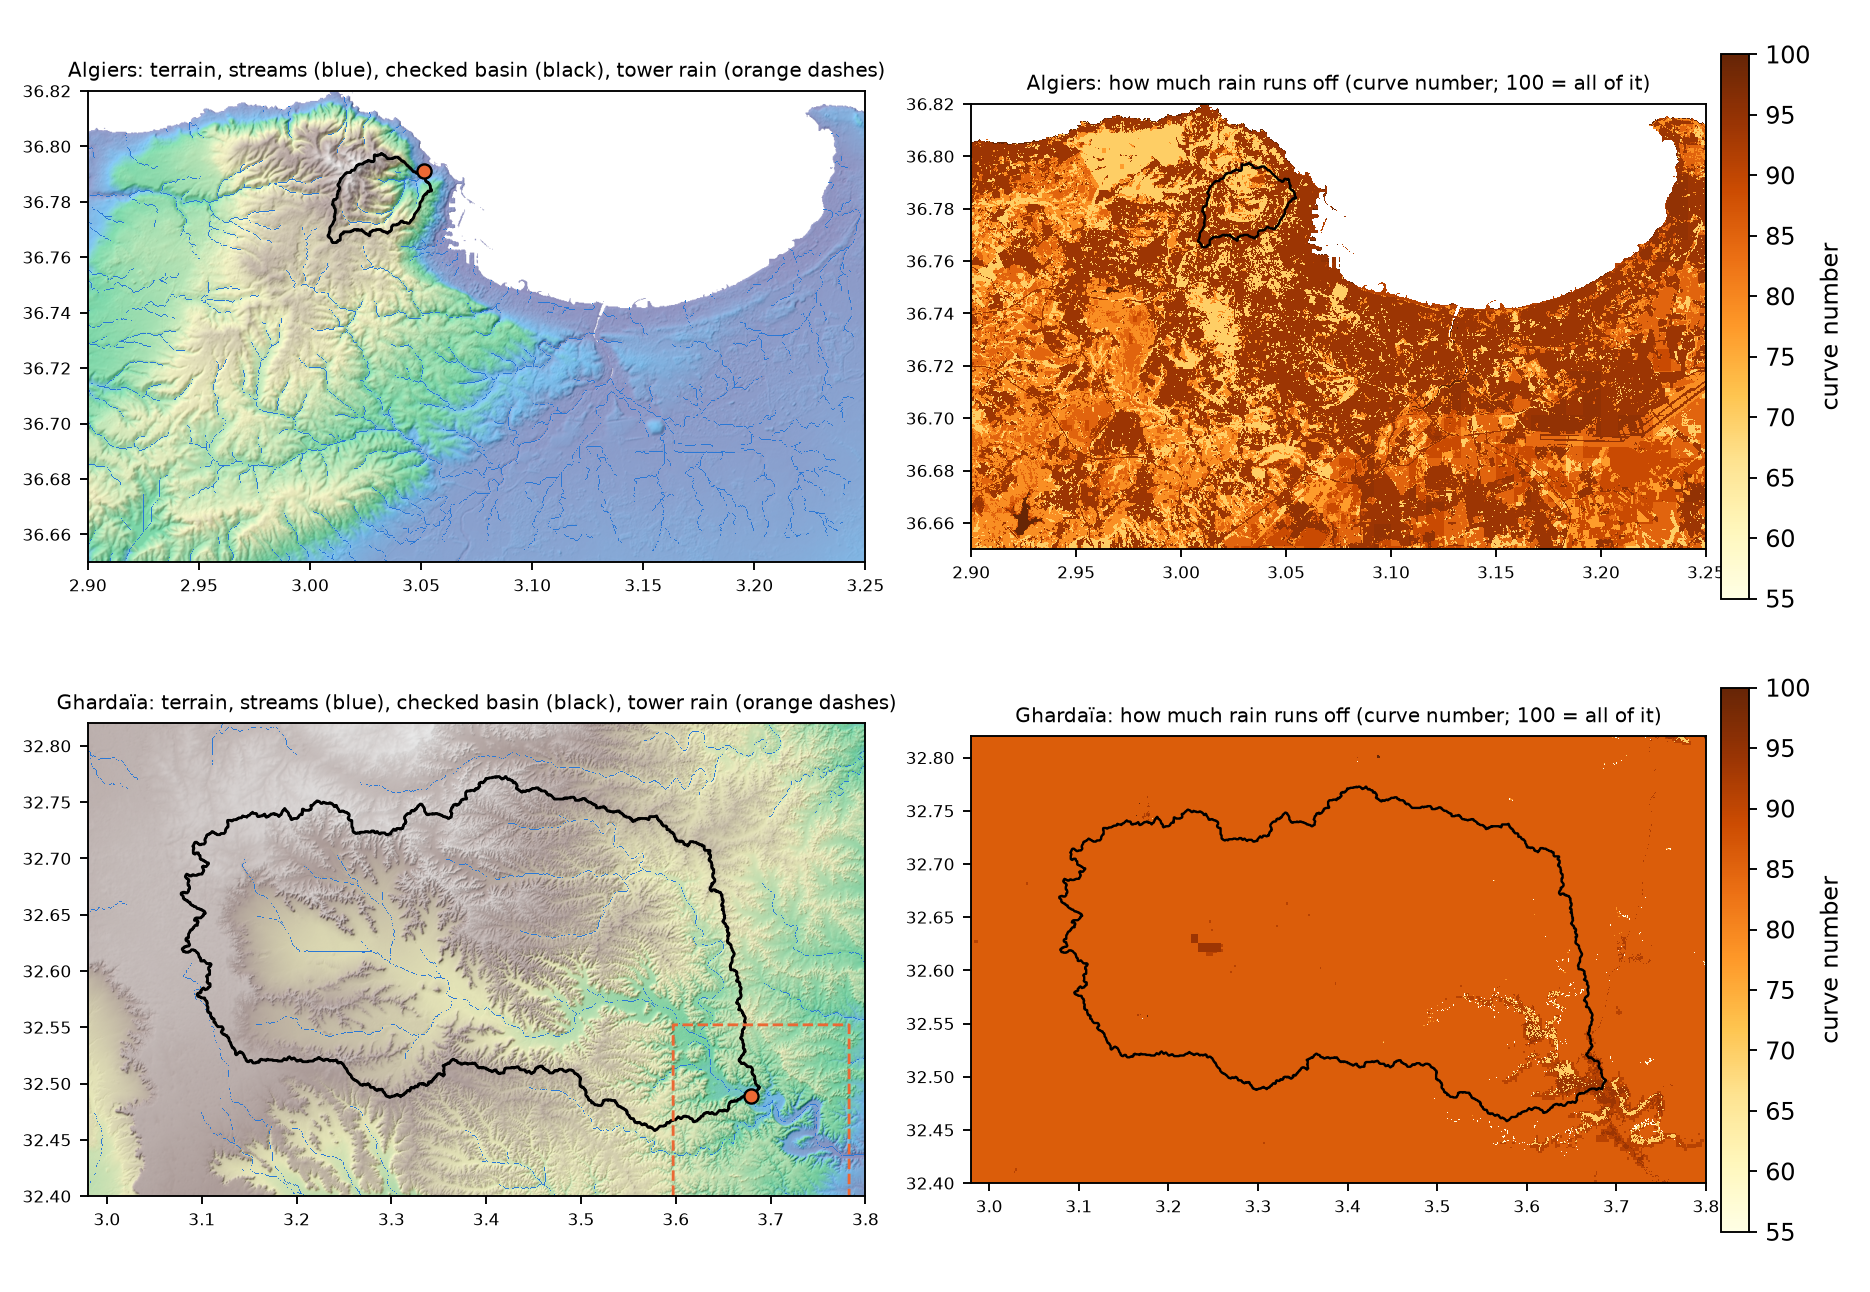
\includegraphics[width=\textwidth]{fig_p5_ground.png}
\caption{The ground. Left: terrain, streams (squares with more than 0.5\,km\textsuperscript{2} upstream in Algiers,
20\,km\textsuperscript{2} in Ghardaïa) and the checked basin. The orange dashes mark the box where Part~4 has tower rain.
Right: the curve number (next section), the share of rain that can run off. Concrete and rock are dark, woods are light.}
\label{fig:p5_ground}
\end{figure}

\begin{careful}
\textbf{The towers cover only the town.} In Ghardaïa the tower rain of Part~4 covers only \PfiveGhaTowerShare{} of the
M'zab basin: the town has towers, the empty plateau upstream does not. Over the rest of the basin, every version of the
storm uses the satellite. This is not a quirk of the simulation. A desert wadi floods from rain that falls far from any
phone mast, so towers alone cannot see a wadi flood coming. In Algiers the towers cover all of Koriche (\PfiveAlgTowerShare).
\end{careful}

%==========================================================
\section{What soaks in: the curve number}
\label{sec:p5_cn}
%==========================================================
Engineers have a simple, well-tested rule for how much of a storm runs off, from the US Soil Conservation Service. Each
piece of ground gets a \textbf{curve number} CN, between 30 (deep sand under forest) and 100 (water, concrete). From it
come the soil's storage $S$ and the first rain it swallows completely, $I_a$:
\begin{equation}
S = \frac{25\,400}{\text{CN}} - 254 \ \text{mm}, \qquad I_a = 0.2\,S, \qquad
Q = \frac{(P - I_a)^2}{P - I_a + S}\ \ \text{for } P > I_a\ (\text{else } Q = 0)
\end{equation}
$P$ is the rain fallen since the storm began and $Q$ the part that has run off. Both are in millimetres.

\begin{example}[: 100 mm on a field]
A field with CN = 80 gets 100\,mm. $S = 25\,400/80 - 254 = 63.5$\,mm and $I_a = 12.7$\,mm, so
$Q = 87.3^2/(87.3 + 63.5) = 50.5$\,mm. Half the rain runs off. With CN = 95 (built-up):
$S = 13.4$, $I_a = 2.7$, $Q = 84.5$\,mm.
\end{example}

The curve number comes from a table, by land cover and soil group (the US standard tables, paired as in the GCN250 world
map). Built-up land has CN 89--95, crops 67--89, woods 30--77 and bare desert ground 77--94. The model applies the rule in
every square at every time step, so a square that has already had a lot of rain runs off more of the next drop.
\begin{itemize}
\item \textbf{Koriche:} average CN \PfiveAlgCN; \PfiveAlgBuilt{} of the basin is built-up.
\item \textbf{M'zab:} average CN \PfiveGhaCN, mostly bare rock and thin stony soil.
\end{itemize}

%==========================================================
\section{Moving the water}
\label{sec:p5_solver}
%==========================================================
The runoff now has to move. We use the method of the reference flood model LISFLOOD-FP: the \textbf{local-inertial
equations} (Bates et al.\ 2010; de Almeida et al.\ 2012). Rain falls on every square (\textbf{rain-on-grid}). Between
every pair of neighbouring squares, the flow is updated many times a minute:
\begin{equation}
q_{\text{new}} = \frac{q - g\,h\,\Delta t\,\dfrac{\Delta\eta}{\Delta x}}{1 + g\,\Delta t\,n^2\,|q|\,/\,h^{7/3}}
\end{equation}
In words:
\begin{itemize}
\item $q$ is the flow across the shared edge, per metre of edge.
\item The top line says that water speeds up towards the lower water surface ($\Delta\eta$ is the difference in water
level, $\Delta x$ the distance, $g = 9.81$\,m/s\textsuperscript{2} gravity, $h$ the water depth at the edge).
\item The bottom line is friction, which slows it down. Rough ground has a high \textbf{Manning's $n$}: 0.03 for bare
ground, 0.10 for woods. On 30-m squares the buildings themselves are not drawn, so built-up land gets $n = 0.05$ to stand
for their drag. We test 0.02 and 0.10 below.
\item Each square's depth then changes by what flowed in minus what flowed out.
\end{itemize}
The time step $\Delta t$ (at most 2 seconds) is set by how fast a wave can travel in the deepest water. Water reaching the
sea leaves the model. Two safety rules are standard: no square can send out more water than it holds, and the speed is
held below the speed of a surface wave.

We wrote the solver ourselves, about 200 lines in PyTorch, so that it runs on the same graphics card as the AI. It
passes four checks with known answers:
\begin{itemize}
\item a lake at rest stays at rest;
\item steady rain on a tilted plane comes out at the bottom at exactly the rate it falls;
\item the textbook curve-number example above;
\item every drop is accounted for. Rain in = soaked in + reached the sea + left at the edges + still on the ground, to
within $\PfiveAlgBudgetErr$ of the runoff in Algiers.
\end{itemize}
A two-day storm over Algiers (\PfiveAlgCells{} million squares, about 100{,}000 time steps) takes about two minutes on one
graphics card. So the model could run in real time with plenty of room to spare.

%==========================================================
\section{Two versions of each storm}
\label{sec:p5_versions}
%==========================================================
Part~4 warned that a 10-km satellite square averages the downpour over a whole district. For a flood this matters a lot:
\begin{itemize}
\item \textbf{Algiers.} Over Koriche the simulated storm brings \PfiveAlgStormSat\,mm in two days. The rain gauge at
Bouzaréah, on the ridge above the basin, measured \PfiveAlgGaugeTotal\,mm in 15 hours, including two bursts of about
55\,mm in half an hour.
\item \textbf{Ghardaïa.} Over the M'zab basin the simulated storm brings \PfiveGhaStormSat\,mm. The town recorded about
\PfiveGhaGaugeTotal\,mm over the two days.
\end{itemize}
So we run every flood twice:
\begin{enumerate}
\item \textbf{As the satellite saw it.} Every rain map exactly as in Part~4. This is the fair test of towers against
truth.
\item \textbf{Matched to the gauge.} Every rain map (truth, AI, classical, satellite) multiplied by the same number, so
that the true storm total over the basin equals the gauge: $\times$\PfiveAlgFactor{} in Algiers and $\times$\PfiveGhaFactor{}
in Ghardaïa. The timing and the pattern stay those of the satellite. This is the fair test of the flood model against
the real floods, and a harder test for the towers (bigger rain, bigger errors).
\end{enumerate}

%==========================================================
\section{Does the flood model get the real floods right?}
\label{sec:p5_check}
%==========================================================
First the flood model on its own, driven by the true rain of the gauge-matched storm. The figure shows the flow out of
each checked basin.

\begin{figure}[h]
\centering
\begin{tikzpicture}
\begin{groupplot}[group style={group size=1 by 2,vertical sep=1.5cm},
  width=0.95\textwidth,height=4.6cm,grid=major,grid style={inkc!12},ymin=0,
  tick label style={font=\small},label style={font=\small},
  legend style={font=\scriptsize,draw=none,fill=white,fill opacity=0.85,text opacity=1,at={(0.01,0.97)},anchor=north west},
  legend cell align=left]
\nextgroupplot[ylabel={m\textsuperscript{3}/s},xmin=0,xmax=54,xtick={0,6,12,18,24,30,36,42,48,54},
  xlabel={Algiers, Oued Koriche: hours since 9 Nov 2001 00:00 UTC},ymax=160]
  \addplot[thick,color=inkc] table[x=hour,y=truth] {p5_q_algiers_gauge.dat}; \addlegendentry{true rain}
  \addplot[thick,color=rainc] table[x=hour,y=ai] {p5_q_algiers_gauge.dat}; \addlegendentry{towers + AI}
  \addplot[thick,color=gaugec] table[x=hour,y=classical] {p5_q_algiers_gauge.dat}; \addlegendentry{towers, classical}
  \addplot[thick,color=inkc!45,dashed] table[x=hour,y=imerg] {p5_q_algiers_gauge.dat}; \addlegendentry{satellite only}
  \addplot[thin,color=gaugec,densely dotted,domain=0:54] {143}; \addlegendentry{flood marks, 2001 (143)}
\nextgroupplot[ylabel={m\textsuperscript{3}/s},xmin=0,xmax=84,xtick={0,12,24,36,48,60,72,84},
  xlabel={Ghardaïa, Oued M'zab: hours since 29 Sep 2008 00:00 UTC},ymax=1700]
  \fill[gaugec,opacity=0.12] (axis cs:0,900) rectangle (axis cs:84,1600);
  \node[font=\scriptsize,color=gaugec!80!black,anchor=north east] at (axis cs:83,1590) {reported, 2008};
  \addplot[thick,color=inkc] table[x=hour,y=truth] {p5_q_ghardaia_gauge.dat};
  \addplot[thick,color=rainc] table[x=hour,y=ai] {p5_q_ghardaia_gauge.dat};
  \addplot[thick,color=gaugec] table[x=hour,y=classical] {p5_q_ghardaia_gauge.dat};
  \addplot[thick,color=inkc!45,dashed] table[x=hour,y=imerg] {p5_q_ghardaia_gauge.dat};
\end{groupplot}
\end{tikzpicture}
\caption{Flow out of the checked basin through the gauge-matched storm (10-minute means), for each rain source. Top:
Koriche, with the 143\,m\textsuperscript{3}/s from the 2001 flood marks. Bottom: M'zab; the shaded band is the
900--1{,}600\,m\textsuperscript{3}/s reported for 2008. In Ghardaïa the four lines lie on top of each other.}
\label{fig:p5_hydro}
\end{figure}

\textbf{Algiers.} Out of Koriche come \PfiveAlgGTruthVol{} million m\textsuperscript{3} of water. The flood marks give
\PfiveAlgObsVol{} million: the volume is right. The peak is not:
\begin{itemize}
\item Our model: \PfiveAlgGTruthPeak\,m\textsuperscript{3}/s.
\item The flood marks: \PfiveAlgObsPeak\,m\textsuperscript{3}/s. Menad et al.\ judge \PfiveAlgObsLo--\PfiveAlgObsHi{}
plausible, and their own model gave \PfiveAlgObsModel.
\end{itemize}
Three things in our set-up flatten the peak:
\begin{enumerate}
\item \textbf{Hourly rain.} The two half-hour bursts of about 110\,mm/h become hourly averages, half as intense.
\item \textbf{30-m squares.} The narrow, steep streets that carried the torrent are blurred into wider, rougher squares.
\item \textbf{Clear water.} Our water carries no mud. In 2001 about 30\% of what came down was mud and rubble, which
moves as a heavier, faster mass.
\end{enumerate}
The timing is the satellite's. The gauge-matched storm peaks at \PfiveAlgGTruthPeakTime, because scaling up the night's
rain makes the night the worst part. With the satellite-strength storm the peak comes at \PfiveAlgSTruthPeakTime, the
morning the real flood struck.

\textbf{Ghardaïa.} The M'zab peaks at \PfiveGhaGTruthPeak\,m\textsuperscript{3}/s. The reported values run from
\PfiveGhaObsLo{} to \PfiveGhaObsHi\,m\textsuperscript{3}/s. That is lower, as it should be: in 2008 a dam broke upstream
and is said to have added more than 900\,m\textsuperscript{3}/s, and sediment had raised the wadi bed by up to 1.5\,m. We
model neither. Our peak is close to the estimated 100-year flood of the wadi (722\,m\textsuperscript{3}/s). With the
satellite-strength storm the town starts to flood at \PfiveGhaSTruthFlood{}. That matches the real flood, which came at
dawn on 1 October.

\subsection{Which choices matter?}
The same run (true rain, gauge-matched), with one choice changed at a time:
\begin{center}\footnotesize
\begin{tabular}{lcc}
\toprule
change & Koriche peak (m\textsuperscript{3}/s) & M'zab peak (m\textsuperscript{3}/s)\\
\midrule
none (the runs above) & \PfiveAlgGTruthPeak & \PfiveGhaGTruthPeak\\
soil already wet (moisture class III) & \PfiveAlgSensWet{} (\PfiveAlgSensWetErr) & \PfiveGhaSensWet{} (\PfiveGhaSensWetErr)\\
soil dry (moisture class I) & \PfiveAlgSensDry{} (\PfiveAlgSensDryErr) & \PfiveGhaSensDry{} (\PfiveGhaSensDryErr)\\
pits not filled & \PfiveAlgSensUnfilled{} (\PfiveAlgSensUnfilledErr) & \PfiveGhaSensUnfilled{} (\PfiveGhaSensUnfilledErr)\\
built-up roughness 0.02 instead of 0.05 & \PfiveAlgSensSmooth{} (\PfiveAlgSensSmoothErr) & \PfiveGhaSensSmooth{} (\PfiveGhaSensSmoothErr)\\
built-up roughness 0.10 & \PfiveAlgSensRough{} (\PfiveAlgSensRoughErr) & \PfiveGhaSensRough{} (\PfiveGhaSensRoughErr)\\
city drains take 20\,mm/h & \PfiveAlgSensDrains{} (\PfiveAlgSensDrainsErr) & --\\
\bottomrule
\end{tabular}
\end{center}
\begin{itemize}
\item \textbf{Roughness and pit filling barely matter in the city.} Our main approximations are safe there.
\item \textbf{The soil matters, above all in the desert.} The same storm on wet or dry ground changes the M'zab peak from
\PfiveGhaSensDry{} to \PfiveGhaSensWet\,m\textsuperscript{3}/s. A real warning system must track how wet the ground is,
as the WMO flash-flood system does.
\item \textbf{Drains matter most in the city.} Working drains of 20\,mm/h would have more than halved the Koriche peak.
In 2001 the drains were reported blocked, which is why the default has none. We do not have the sewer map (it is not
public).
\end{itemize}

%==========================================================
\section{Does tower rain give the same flood?}
\label{sec:p5_towers}
%==========================================================
Now the real question. Each flood is run again with each rain source, and compared with the run on the true rain:
\begin{itemize}
\item \textbf{peak} and \textbf{volume}: the flow out of the basin;
\item \textbf{flooded built-up land}: the overlap between the built-up squares that get 30\,cm or more in both runs and in
either run (1 = the same squares);
\item \textbf{commune ranking}: do the same communes come out most at risk? This is the rank correlation of each
commune's built-up hectares in significant or extreme danger (1 = same order).
\end{itemize}

\begin{center}\footnotesize\setlength{\tabcolsep}{4pt}
\begin{tabular}{llcccc}
\toprule
storm & rain used & Koriche peak & Koriche volume & flooded built-up land & commune ranking\\
\midrule
gauge-matched & towers + AI & \PfiveAlgGAIPeakErr & \PfiveAlgGAIVolErr & \PfiveAlgGAICSI & \PfiveAlgGAISpear\\
 & towers, classical & \PfiveAlgGClPeakErr & \PfiveAlgGClVolErr & \PfiveAlgGClCSI & \PfiveAlgGClSpear\\
 & 3\% of towers + AI & \PfiveAlgGSparsePeakErr & \PfiveAlgGSparseVolErr & \PfiveAlgGSparseCSI & \PfiveAlgGSparseSpear\\
 & satellite only & \PfiveAlgGSatPeakErr & \PfiveAlgGSatVolErr & \PfiveAlgGSatCSI & \PfiveAlgGSatSpear\\
\midrule
satellite-strength & towers + AI & \PfiveAlgSAIPeakErr & \PfiveAlgSAIVolErr & \PfiveAlgSAICSI & \PfiveAlgSAISpear\\
 & towers, classical & \PfiveAlgSClPeakErr & \PfiveAlgSClVolErr & \PfiveAlgSClCSI & \PfiveAlgSClSpear\\
 & 3\% of towers + AI & \PfiveAlgSSparsePeakErr & \PfiveAlgSSparseVolErr & \PfiveAlgSSparseCSI & \PfiveAlgSSparseSpear\\
 & satellite only & \PfiveAlgSSatPeakErr & \PfiveAlgSSatVolErr & \PfiveAlgSSatCSI & \PfiveAlgSSatSpear\\
\bottomrule
\end{tabular}

\smallskip
{\footnotesize Algiers. Peak and volume: difference from the run on the true rain. Flooded built-up land and commune
ranking: agreement with that run (1 = perfect).}
\end{center}

\begin{figure}[h]
\centering
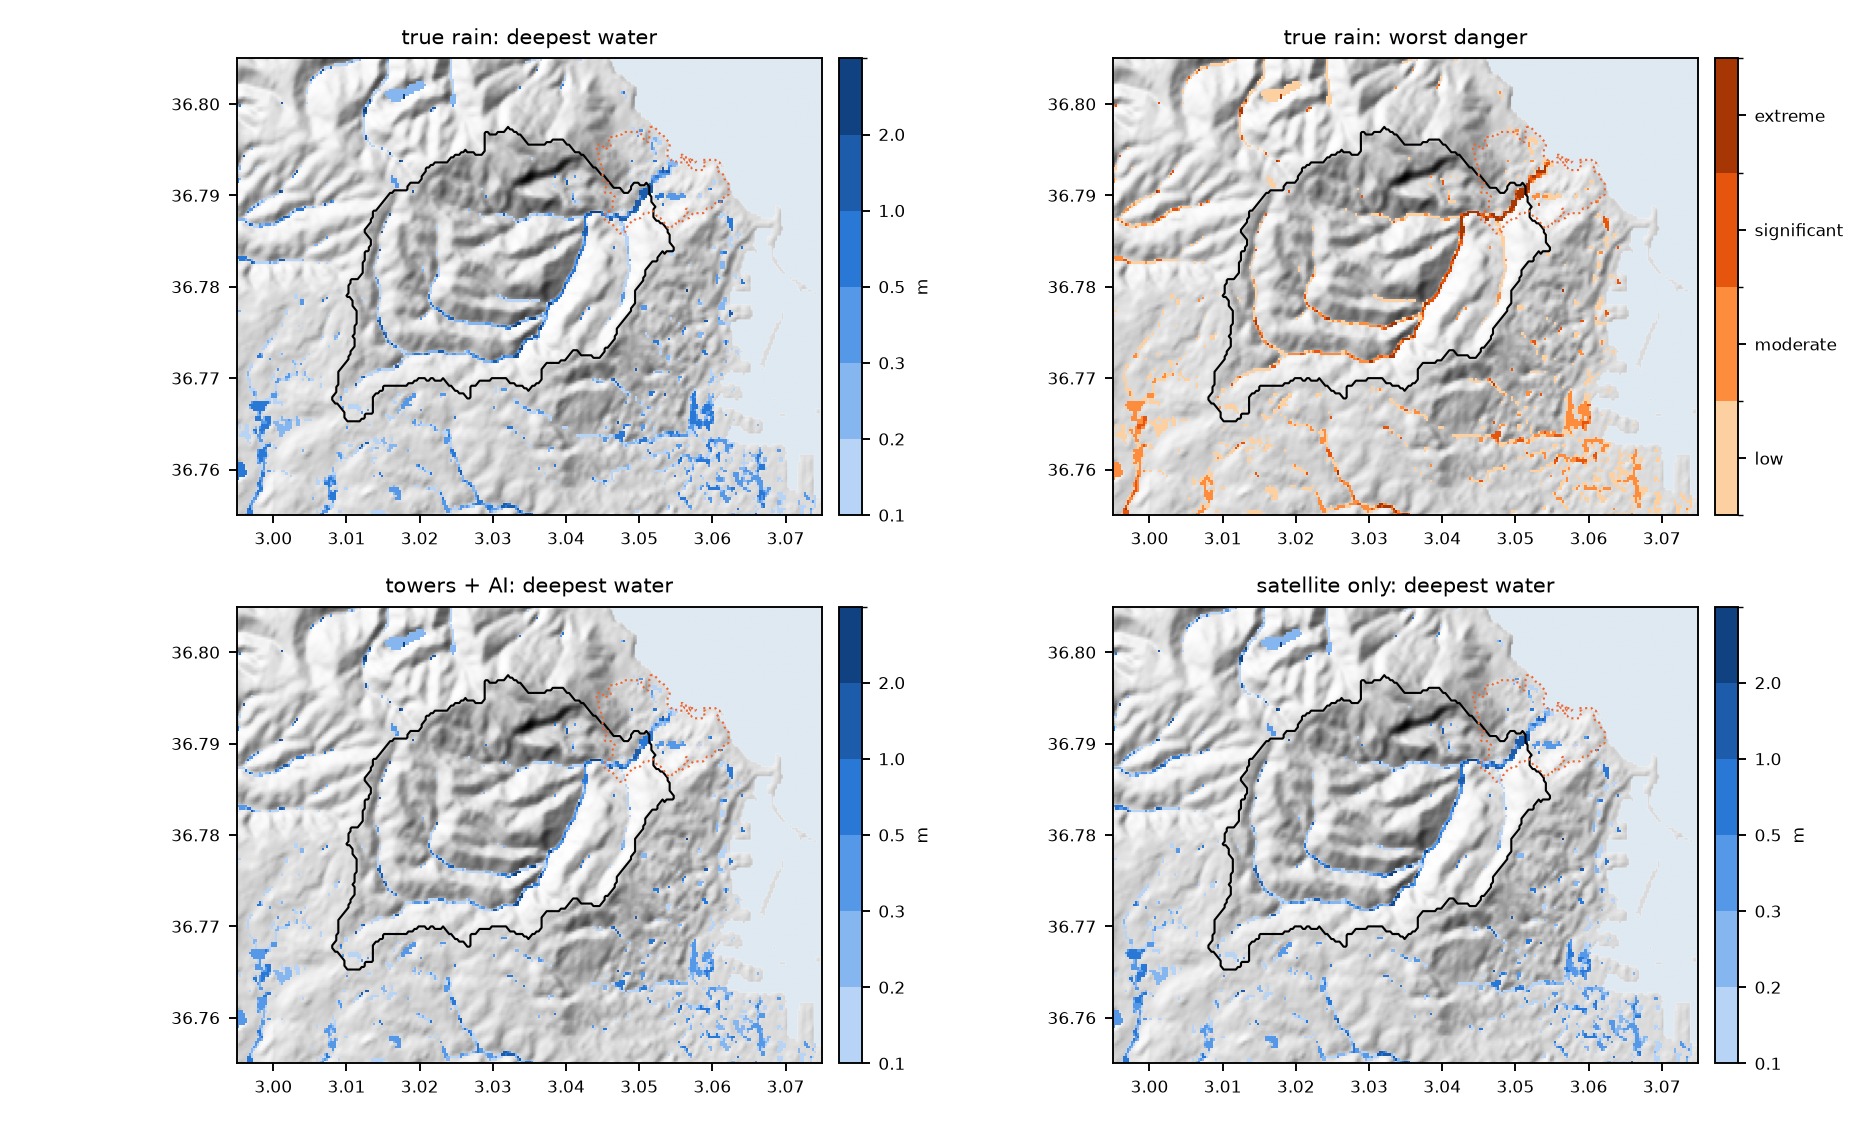
\includegraphics[width=\textwidth]{fig_p5_flood_algiers.png}
\caption{Koriche and Bab El Oued, gauge-matched storm. Top: the deepest water and the worst danger with the true rain.
Bottom: the deepest water with tower + AI rain, and with satellite rain only. Black: the Koriche basin. Orange dots: the
commune of Bab El Oued, where the alarm is judged. The same streets fill in every run; with AI rain they fill less.}
\label{fig:p5_flood_alg}
\end{figure}

\begin{itemize}
\item \textbf{Where the water goes, tower rain gets right.} The flooded built-up land overlaps \PfiveAlgGClCSI{}
(classical) and \PfiveAlgGAICSI{} (AI) with the true run. The commune ranking agrees at \PfiveAlgGClSpear{} and
\PfiveAlgGAISpear. That is natural: the terrain decides where water collects, and the rain decides only how much. With
the true rain, the communes with the most built-up land in danger are \PfiveAlgCommuneA{} (\PfiveAlgCommuneAHa\,ha, on
the low plain of the Oued El Harrach), \PfiveAlgCommuneB{} and \PfiveAlgCommuneC.
\item \textbf{How much water, the AI gets badly wrong.} The AI map's rain was off by \PfourAlgAIMapBias{} in Part~4; here its flood peak is off by
\PfiveAlgGAIPeakErr. A flood magnifies rain errors, for two reasons. The curve number
keeps the first millimetres of every storm, so a smaller storm loses a larger share. And peaks come from the heaviest
hours, exactly where the AI under-measures most (Part~4). The classical method's peak is off by \PfiveAlgGClPeakErr.
\item \textbf{A few towers do about as badly as all of them} (\PfiveAlgGSparsePeakErr): the shortfall comes from the
AI, not from the number of links.
\item \textbf{In Ghardaïa every source gives the same wadi flood} (peaks within 1\%). The towers cover only
\PfiveGhaTowerShare{} of the basin, so it is the satellite's rain upstream that makes the flood.
\end{itemize}

\begin{careful}
\textbf{The satellite looks far better here than it is.} The simulated truth was built \emph{from} the satellite: its
10-km amounts were kept exactly (Part~4, Step~3). So ``satellite only'' is right by construction at 10\,km, and it misses
only the detail inside each square. In reality the satellite's error is far larger. Over Koriche it saw
\PfiveAlgStormSat\,mm where the Bouzaréah gauge measured \PfiveAlgGaugeTotal\,mm. This simulation cannot show that
weakness. What it can show fairly is \emph{time}, which comes next.
\end{careful}

%==========================================================
\section{Would the alarm have come in time?}
\label{sec:p5_warn}
%==========================================================
A warning is useful only if it comes before the water. We test two ways of raising one.

\textbf{1. Rain thresholds (flash-flood guidance).} This is how the WMO's Flash Flood Guidance System works. For each
duration we find the rain that is just enough to flood the town, by running made-up storms (the same rain everywhere)
of growing size through the flood model. ``Flooding the town'' means \PfiveAlgAlarmHa{} hectares of built-up land under
30\,cm of water. The alarm sounds when the measured rain over the town, or over the basin, passes the threshold for any
duration.
\begin{center}\footnotesize
\begin{tabular}{lccccc}
\toprule
rain in & 1 hour & 3 hours & 6 hours & 12 hours & 24 hours\\
\midrule
floods Bab El Oued & \PfiveAlgThrA\,mm & \PfiveAlgThrB\,mm & \PfiveAlgThrC\,mm & \PfiveAlgThrD\,mm & \PfiveAlgThrE\,mm\\
floods Ghardaïa & -- & \PfiveGhaThrA\,mm & \PfiveGhaThrB\,mm & \PfiveGhaThrC\,mm & \PfiveGhaThrD\,mm\\
\bottomrule
\end{tabular}
\end{center}

\textbf{2. Running the flood model on the rain as it arrives.} The model runs more than 1{,}000 times faster than real time (two days of storm in about two
minutes), so it could run continuously. The alarm is the moment it shows the town flooding.

Either way, the rain has to reach us first. Towers report every minute, so we allow 5 minutes. NASA publishes its first
satellite estimate (IMERG Early) about 4 hours after the rain, so we allow 4 hours.

\begin{center}\footnotesize\setlength{\tabcolsep}{4pt}
\begin{tabular}{lcccc}
\toprule
& \multicolumn{2}{c}{gauge-matched storm} & \multicolumn{2}{c}{satellite-strength storm}\\
\cmidrule(lr){2-3}\cmidrule(lr){4-5}
rain used & rain threshold & flood model & rain threshold & flood model\\
\midrule
true rain (no delay) & \PfiveAlgGTruthLead & -- & \PfiveAlgSTruthLead & --\\
towers + AI & \PfiveAlgGAILead & \PfiveAlgGAIModelLead & \PfiveAlgSAILead & \PfiveAlgSAIModelLead\\
towers, classical & \PfiveAlgGClLead & \PfiveAlgGClModelLead & \PfiveAlgSClLead & \PfiveAlgSClModelLead\\
3\% of towers + AI & \PfiveAlgGSparseLead & \PfiveAlgGSparseModelLead & \PfiveAlgSSparseLead & \PfiveAlgSSparseModelLead\\
satellite only & \PfiveAlgGSatLead & \PfiveAlgGSatModelLead & \PfiveAlgSSatLead & \PfiveAlgSSatModelLead\\
\bottomrule
\end{tabular}

\smallskip
{\footnotesize Bab El Oued: alarm time compared with the moment the town floods in the true run (gauge-matched:
\PfiveAlgGTruthFlood; satellite-strength: \PfiveAlgSTruthFlood). ``Early'' is warning time; ``late'' means the streets
were already under water.}
\end{center}

\begin{itemize}
\item \textbf{The delay of the data decides.} With the same flood model, satellite rain arrives \PfiveAlgGSatModelLead{}
in the gauge-matched storm. Classical tower rain gives \PfiveAlgGClModelLead{}, AI tower rain \PfiveAlgGAIModelLead. Four
hours of delay cannot be won back. Minutes can.
\item \textbf{But the AI's shortfall costs it the alarm.} In the milder satellite-strength storm, AI rain never shows the
town flooding: a missed warning. The town did flood in the true run (only just over the line). Rain that reads too low
delays or hides the alarm, which is why the shortfall found in Parts~2 and~4 matters most here.
\item \textbf{Thresholds give the earliest warning when they work.} With the true rain they gave \PfiveAlgGTruthLead{} in
the big storm. In the milder storm they came \PfiveAlgSTruthLead, probably because the threshold assumes the same rain
everywhere and this storm was patchier.
\end{itemize}

\textbf{Ghardaïa.} Its threshold is low: \PfiveGhaThrA\,mm, whatever the duration, because the town sits on the wadi
floor where water collects quickly. Every rain source passes it on 29 or 30 September, about a day before
the town floods in the satellite-strength run (\PfiveGhaSTruthFlood). A threshold that fires so early is a false alarm
followed by silence, so a fixed threshold is not good enough in the desert. It must follow how wet the ground is, and be
tuned on real records. Running the flood model on the arriving rain instead puts the AI \PfiveGhaSAIModelLead{} and the
satellite \PfiveGhaSSatModelLead{} (satellite-strength storm). The classical method raises the alarm
\PfiveGhaSClModelLead{}, which is a false alarm: it reads rain from link noise in the town where little fell (Part~4).

\begin{figure}[h]
\centering
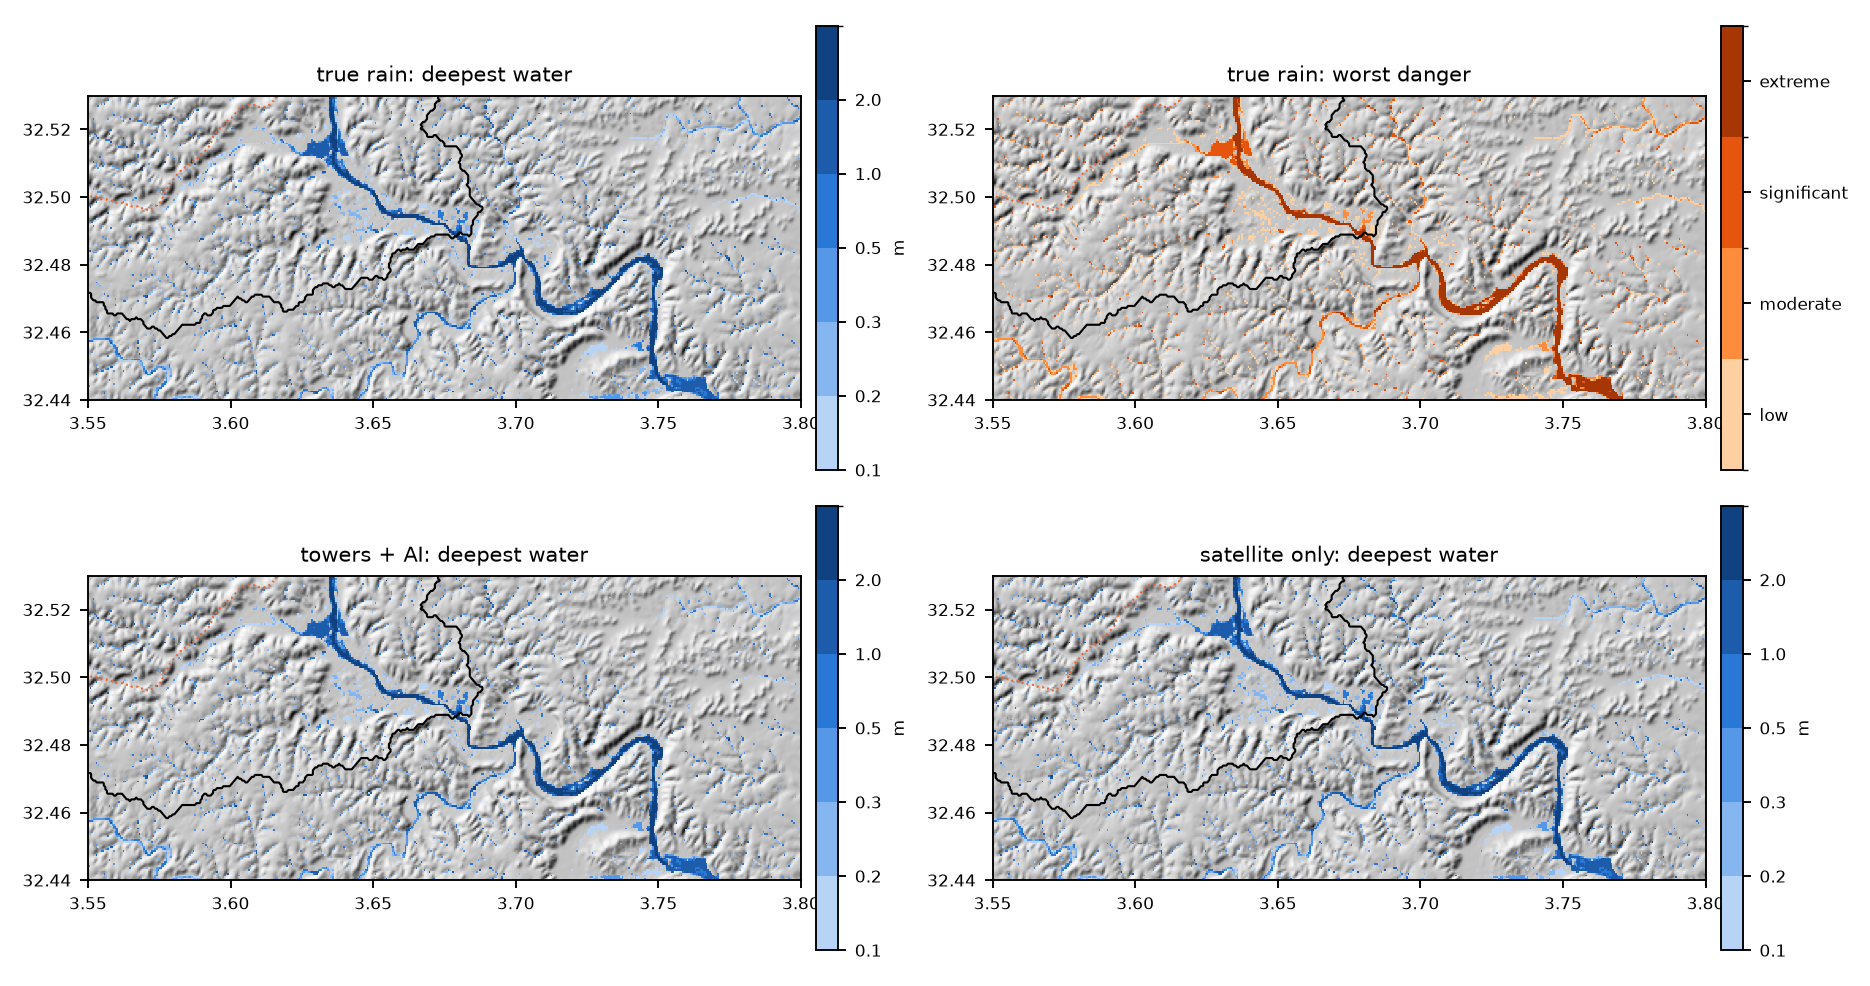
\includegraphics[width=\textwidth]{fig_p5_flood_ghardaia.png}
\caption{The M'zab valley at Ghardaïa, gauge-matched storm (same panels as Figure~\ref{fig:p5_flood_alg}). The wadi fills
the same way whatever the rain source, because the rain that makes it falls upstream, outside the tower area.}
\label{fig:p5_flood_gha}
\end{figure}

\begin{careful}
\textbf{What flatters, and what is harder than reality.}
\begin{itemize}
\item \textbf{Flatters the towers:} everything Part~4 listed (smoothed storms, slowly changing rain, matching physics),
plus a flood model that is itself perfect here. The ``true'' flood comes from the same model, so only the rain differs.
\item \textbf{Flatters the satellite:} the truth keeps its 10-km amounts (box above).
\item \textbf{Harder than reality:} no rain forecast (nowcasting, Part~3, could add 30--60 minutes), and hourly rain maps.
The towers measure every minute, and finer maps would sharpen both the peaks and the alarms.
\item \textbf{Not modelled:} sewers, mud and debris, dam breaks, and changes to the ground since 2001 and 2008 (the
terrain is from 2011--2015, the land cover from 2021).
\end{itemize}
\end{careful}

\begin{oneline}
The flood model reproduces the volume of the 2001 Bab El Oued flood and the timing of the 2008 Ghardaïa flood. Tower rain
puts the floods in the right streets and ranks the communes at risk almost as the true rain does, and it arrives hours
before the satellite's. But the AI's rain shortfall becomes a peak half too low and a delayed or missed alarm, and in a
desert wadi the towers cannot see the rain that matters.
\end{oneline}

%==========================================================
\section{Every choice, and why}
\label{sec:p5_choices}
%==========================================================
\begin{center}\footnotesize\setlength{\tabcolsep}{4pt}
\begin{tabular}{>{\raggedright\arraybackslash}p{2.8cm}>{\raggedright\arraybackslash}p{3.6cm}>{\raggedright\arraybackslash}p{6.9cm}}
\toprule
Choice & Value & Why, and how it was checked\\
\midrule
Flood method & 2D local-inertial, rain on grid & the standard fast method (LISFLOOD-FP); checked on a still lake, a tilted plane and the
water balance\\
Terrain & Copernicus GLO-30, pits filled & free, worldwide; filling barely changes Algiers ($-1\%$), lowers the M'zab peak if not done
($-28\%$)\\
Grid & 30\,m Algiers, 60\,m Ghardaïa & the M'zab basin is 1{,}400\,km\textsuperscript{2}; 60\,m keeps a run under 3 minutes\\
Losses & SCS curve number, moisture class II & standard where soil data is thin; class I and III tested\\
Land cover, soil & WorldCover 10\,m, HYSOGs250m & free, worldwide; dual soil groups taken as D (undrained)\\
Roughness & Manning $n$ by land cover, built-up 0.05 & buildings not resolved at 30\,m; 0.02 and 0.10 tested ($\pm3\%$)\\
Sewers & none (blocked) & reported blocked in 2001; 20\,mm/h tested ($-56\%$)\\
Storm versions & satellite-strength and gauge-matched & the first tests the towers, the second the flood model\\
Rain outside the tower box & satellite & what a real system would have there\\
Hazard & DEFRA rating, 4 classes & standard, uses depth and speed together\\
Town flooded & 5\,ha of built-up land under 30\,cm & knee-deep water over several blocks\\
Rain thresholds & made-up uniform storms, 1--24\,h & the flash-flood guidance idea; uniform rain is its known weakness\\
Data delay & towers 5\,min, satellite 4\,h & tower polling vs IMERG Early publication\\
\bottomrule
\end{tabular}
\end{center}

\textbf{What would make it real.} To turn this simulation into a test, we would need:
\begin{itemize}
\item rain gauge records at 5--15 minutes from the national weather service (ONM) and the water agency (ANRH);
\item flood marks and the sewer map of Algiers (SEAAL);
\item the 2008 satellite flood maps of the International Charter;
\item and, above all, link records from an operator.
\end{itemize}
The whole chain (link records, AI, rain map, flood model, alarm) already runs faster than real time on one graphics card.

\textbf{Next:} Part~6 brings rain, floods and alarms together in one live dashboard.
